\section{Results Analysis - Linear Drag Model}
Prepare yourself, because our hard work has paid off.

\subsection{Test Case: High Drag}
We fit our linear drag model to the same test case as Fig.~\ref{fig:Analysis1_Test4_Fig5_NoDrag}, and the results are shown in Fig.~\ref{fig:Analysis2_Test4_Fig5_LinearDrag}. The position and velocity plots both track very nicely.\footnote{We provide no quantitative analysis of the fit here due to a lack of internalized, intuitive understanding of statistics. I'm not going to show numbers for the sake of showing numbers if they don't mean anything to me. In my professional experience, people have relied on me to judge if the vibes are good or bad without ever asking me for the numbers to prove it.}

The more interesting results are in the frame-by-frame behavior.

\begin{figure}[t]
\centering
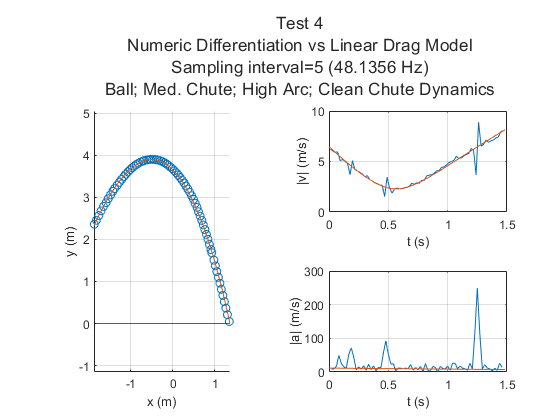
\includegraphics[width=0.9\linewidth]{images/Analysis2_Test4_Fig5_LinearDrag.png}
\caption{\label{fig:Analysis2_Test4_Fig5_LinearDrag} Fitting the linear drag model to sampled position data for a ball with a parachute. Lookin' good. Check out how nice it tracks the velocity plot while rejecting the spikes.}
\end{figure}

\subsection{Test Case: High Drag - Frame by Frame}

\begin{figure*}[t!]
    \centering
    \begin{subfigure}[t]{0.5\textwidth}
        \centering
        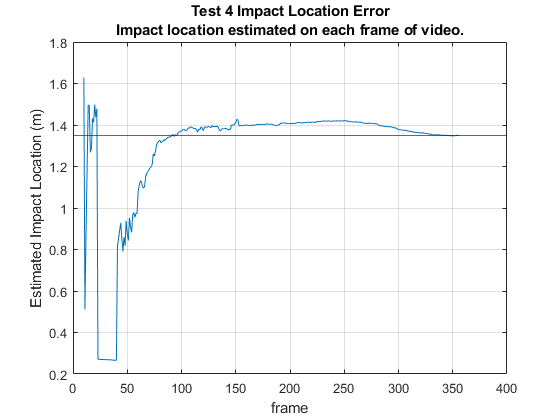
\includegraphics[width=\textwidth]{images/Analysis2_Test4_ImpLocPlot_LinearDrag.png}
        \caption{}
    \end{subfigure}%
    ~ 
    \begin{subfigure}[t]{0.5\textwidth}
        \centering
        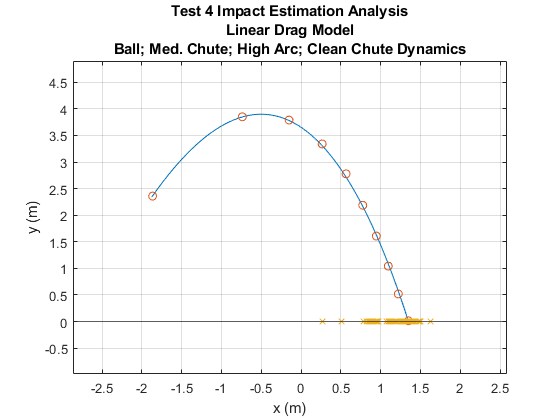
\includegraphics[width=\textwidth]{images/Analysis2_Test4_ImpLocHist_LinearDrag.png}
        \caption{}
    \end{subfigure}
    \caption{\label{fig:Test4_LinearDrag_FrameByFrame} Frame-by-frame impact location estimation for a ball with a parachute using the linear drag model. (a) Impact location over time. (b) Impact locations marked.}
\end{figure*}

\begin{figure}[t]
\centering
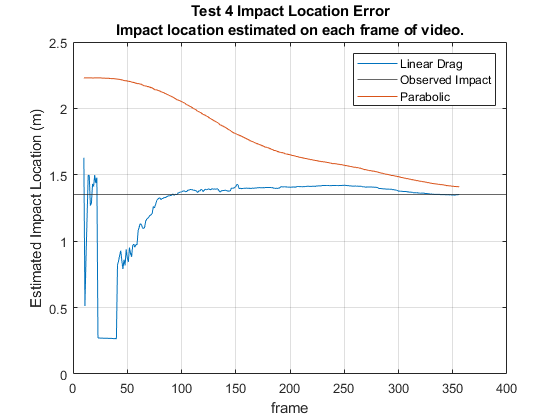
\includegraphics[width=0.9\linewidth]{images/Analysis2_Test4_ImpLocPlot_Both.png}
\caption{\label{fig:Analysis2_Test4_ImpLocPlot_Both} Estimated impact location predicted on each frame of video using the linear aerodynamic drag model (blue) and the parabolic model (orange). The linear drag model is more chaotic in shape, but lower error. We propose that the error in the linear drag model is due mostly to unmodeled multibody dynamics with the parachute.}
\end{figure}

Now Fig.~\ref{fig:Test4_LinearDrag_FrameByFrame} is some data you can sink your teeth into. It's interesting how chaotic the prediction is near the start of the flight, but it does seem to get a decent sense of the impact location around the apex. For the reader's convenience, the results from Fig.~\ref{fig:Test4_NoDrag_FrameByFrame} and Fig.~\ref{fig:Test4_LinearDrag_FrameByFrame} have been plotted together in Fig.~\ref{fig:Analysis2_Test4_ImpLocPlot_Both}. 

It's clear that the linear drag model does much better than the parabolic model. Even though the start is rough at the start, it quickly converges to the correct value and stays within that region. And, importantly, it correctly tracks it down to the moment of impact. This behavior provides a useable basis for a realtime application. The quick convergence would enable a system with high inertia plenty of time to actuate to a required orientation, leaving only minor corrections to be made near the moment of impact. 

At this time we should also propose some explanation for the remaining error. Why isn't it perfect now that we've added the drag model? What's with those discontinuous steps in predicted location? 

First, the general imperfections. There are still some unmodeled dynamics remaining in the system. The parachute-ball system tends to rock and wobble around like a pendulum. Also, we believe the parachute may provide some lift force, in addition to drag force, which would cause it to glide away from a pure drag-based trajectory. These could all throw off the prediction.\footnote{These are just proposed explanations. The analysis to confirm this has not been done.} 

Second, the discontinuities. These are likely an artifact of the interaction between a specific error source in Tracker and the implementation of our Gradient Descent algorithm. When generating the data in Tracker we utilize the Autotracker for as many frames as we can. However, it has a tendency to drift off of the center of the projectile over time. To correct this, the tracking point is manually re-centered every few frames. This creates a discontinuity in the input data. Now recall that the gradient descent algorithm finds the value of the drag coefficient that minimizes the error. If there's a discontinuity in the input, then the best fit drag coefficient will have a discontinuity as well. The earlier into the flight, the larger an impact such a discontinuity would have. This could perhaps be mitigated by rate limiting the drag coefficient, or rate limiting the predicted impact location. 

Finally, we'd also like to note that the parachute does not pull evenly at all times. There is some turbulence near the start of the flight, and the strings often go slack near the apex before the chute whips around as the ball falls. This motion is all not captured by the model. 

Now we'll move on to some application ideas.
